\documentclass[12pt,oneside]{report}

% ---------- Packages ----------
\usepackage[utf8]{inputenc}
\usepackage[T1]{fontenc}
\usepackage{lmodern}
\usepackage{setspace}
\usepackage{geometry}
\geometry{letterpaper, margin=1in}
\usepackage{graphicx}
\graphicspath{{figures/}}
\usepackage{caption}
\usepackage{subcaption}
\usepackage{booktabs}
\usepackage{amsmath, amssymb}
\usepackage[hidelinks]{hyperref}
\usepackage[nameinlink,capitalise]{cleveref}
\usepackage{enumitem}
\usepackage{xcolor}
\usepackage{titlesec}
% Minimal approach - let LaTeX handle TOC normally
\usepackage{csquotes}
\usepackage[style=numeric,natbib=true]{biblatex}

\addbibresource{references.bib}

\setcounter{secnumdepth}{3}
\setcounter{tocdepth}{2}
\onehalfspacing

% Custom chapter formatting - remove "Chapter" prefix and newlines
\titleformat{\chapter}[hang]
{\normalfont\Large\bfseries}{\thechapter}{1em}{}
\titlespacing*{\chapter}{0pt}{0pt}{20pt}

% ---------- Title Info ----------
\newcommand{\proposaltitle}{Deep Learning for Scalable Sensorimotor Brain-Computer Interfaces}
\newcommand{\authorname}{\textbf{Joel Ye}}
\newcommand{\department}{Neural Computation \& Machine Learning}
\newcommand{\university}{Carnegie Mellon University}
\newcommand{\proposaldate}{July 30, 2025}

% ---------- Committee Macro ----------
\newcommand{\committee}{
\begin{itemize}[leftmargin=1.2em]
  \item Robert Gaunt (co-chair)
  \item Leila Wehbe (co-chair)
  \item Jennifer Collinger
  \item Aran Nayebi
  \item Chethan Pandarinath
\end{itemize}
}

% ---------- Convenience ----------
\newcommand{\todo}[1]{\textcolor{red}{TODO: #1}}

% ---------- Document ----------
\begin{document}

\begin{titlepage}
  \centering
  {\LARGE \textbf{\proposaltitle}\par}
  \vspace{1em}
  {\Large Thesis Proposal\par}
  \vspace{2em}
  {\large \authorname\par}
  \vfill
  {\large \department\par}
  {\large \university\par}
  {\large \proposaldate\par}
\end{titlepage}

\pagenumbering{roman}

\section*{Abstract}
\addcontentsline{toc}{section}{Abstract}
The increasing ambition of neuroscience and neurotechnology both entails and requires vast troves of neural data. To operate effectively on neural data at scale, neural data science must in turn develop frameworks that can precisely and robustly model broad and heterogeneous data. This task could potentially be made tractable with deep learning (DL), which in the last decade has not only become a foundational tool in artificial intelligence (AI), but has also seen growing adoption in the natural sciences. This proposal advances this program in the domain of sensorimotor intracortical brain-computer interfaces (iBCI), which seek to connect a user’s neural activity with their bodily state. Currently, by modeling small datasets of paired motor cortical activity and behavioral intention, experimenters can calibrate iBCIs that show remarkable potential in allowing users to control robotic limbs. Analogously, experimenters can also provide targeted tactile sensations by applying intracortical microstimulation (ICMS) to somatosensory cortex. However, real-world adoption of sensorimotor BCIs will require translating this potential into a system that is exquisitely reliable and convenient.
The challenge of building such a system is precisely that of operating effectively on BCI data at scale.
% That is, by reframing the accumulation of BCI datasets throughout device lifetime not as standalone snapshots but as a landscape of related data,
% deep learning becomes an  provide a tractable platform with which to encapsulate this landscape.
Therefore, this challenge might be best met with deep learning models that encapsulate the landscape of data accumulated throughout the BCI device's lifetime.
%  reframe BCI data not as a collection of standalone datasets but as a store of related data accumulated throughout the BCI device's lifetime.
I next introduce one result and two proposed works that build this case.

\textbf{Aim 1: Large scale pretraining improves modeling of intracortical motor datasets [in submission].}

The driver of deep learning’s efficacy across domains is its ability to leverage conserved statistical structure across datasets, primarily enabled by a stage of model preparation on large scale data called pretraining. Previous work has identified the requisite conserved structures across neural datasets of motor behavior, and so we systematically measure the efficacy of deep neural network (DNN) pretraining on motor BCI datasets. We establish that DNN efficacy improves with neural data scale on both multi-subject and multi-behavior motor cortical datasets. Yet, this scaling has diminishing returns as data in the downstream, target setting grows, rendering the scaling less impactful for long term BCI applications. This shows pretrained networks may accelerate BCI calibration speeds but will not fundamentally remove the need for continuous BCI data collection.

\textbf{Aim 2: Pretrained deep networks enable continuous and scaleable upper limb neuroprosthetic control. [proposed].}

High degree of freedom control of a robotic arm and hand is possible with current iBCI hardware, but current decoders require extensive daily recalibration and still far underperform able bodied control. Based on successful deep network use in speech BCIs, we propose that an NDT-based controller (NDT3o) which accumulates calibration data across days can address both of these challenges. We will evaluate NDT3o for 7-degree of freedom neuroprosthetic arm and hand control in up to two human participants, aiming to demonstrate continuous high performance in functional tasks of upper limb control. We further aim to illustrate the model’s scalability by extending this control to additional degrees of freedom in the hand without changes to the model design.

\textbf{Aim 3: Modeling intracortical microstimulation for sensory BCIs. [proposed].}

Sensory feedback is integral to native motor control, and can be provided in iBCIs through intracortical microstimulation (ICMS) of the somatosensory cortex. The sensory feedback provided by ICMS can improve BCI control, but our understanding of how ICMS accomplshes this through its modulation of ongoing neural activity is poor. Specifically, we lack a predictive model of the neural response to ICMS, which precludes the development of any sophisticated ICMS protocols. Towards this goal, we first introduce a method to recover spiking activity from artifacted recordings, and then taxonomize the sensory neural response to ICMS through DNN transfer learning expeirments. In this taxonomy, we show that while deep networks largely generalize to temporal variety in stimulation patterns, they fail to generalize to new stimulation channels, showing channel-specific idiosyncrasy in the neural response to ICMS.

% Table of contents
\tableofcontents

\cleardoublepage
\pagenumbering{arabic}

% =========================
% Introduction
% =========================
\chapter{Introduction and Background}

\begin{figure}[h]
  \centering
  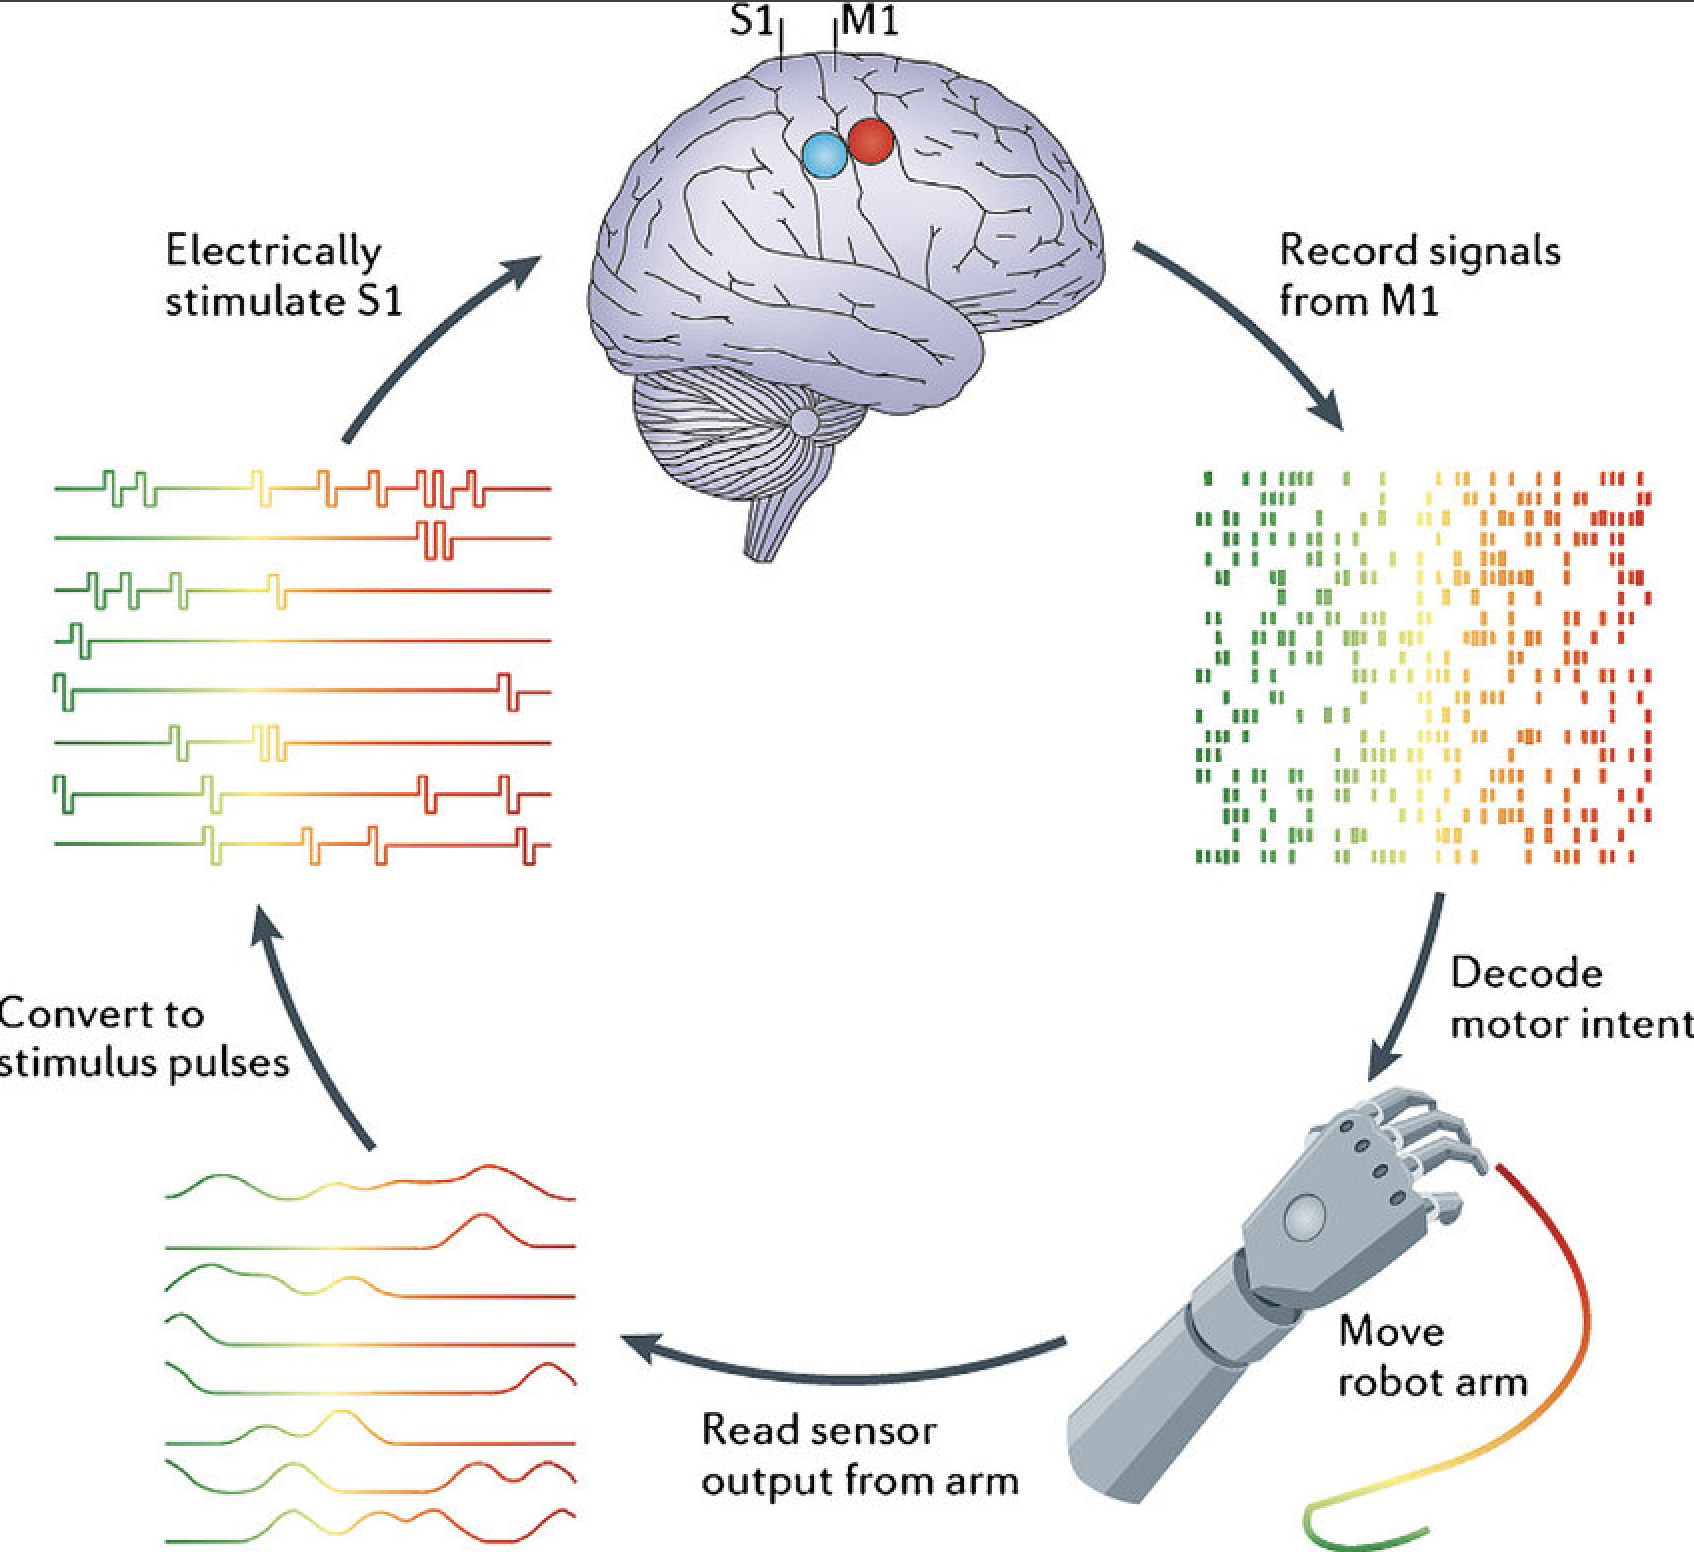
\includegraphics[width=0.5\linewidth]{ch1_bci_loop.png}
  \caption{Will probably redraw this for more aesthetic simplicity, but this is basically what I want to show.}
  \label{fig:bci_loop}
\end{figure}

Today, neuroscientists seek to study the brain in natural, dynamic environments, and neurotechnology companies are similarly racing to produce a device that will work robustly in the real world. The challenge of modeling even a fraction of the brain within this broad scope resists specific definition because it is a problem of a thousand cuts. The neural data we study in iBCIs---namely the spiking activity of single neurons in small volumes of human cortex---are affected by innumerable factors. These factors stem from the fact that the recorded neurons are nestled in a highly interconnected biological network that changes on many timescales, and their activity only arrives to our models after passing through several layers of BCI hardware and software. When these factors are stable, the connection between neural data and behavior can appear remarkably straightforward, motivating the use of simple and interpretable models. However, when these factors shift, unobserved to us, the performance of our models can quickly degrade. Regardless of one’s philosophy on whether we can exhaustively characterize these factors and ultimately understand the data we collect, we undoubtedly should expect to continuously evaluate and update our models as we expand the scope of their application. To minimize the Sisyphean burden of this task, many domains faced with similar challenges have turned to deep neural networks, deprioritizing interpretable theories in favor of a data-centric view of modeling, where the role of the model is to capture and interface with the underlying domain data (\cref{fig:bci_schema}).

\begin{figure}[h]
  \centering
  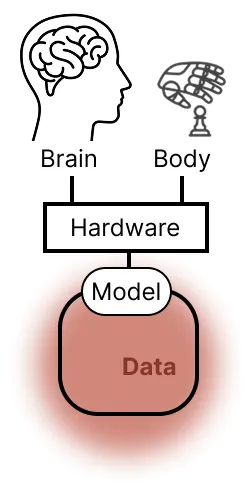
\includegraphics[width=0.5\linewidth]{ch1_bci_schema.png}
  \caption{The role of a computational model is to provide an interface to interact with the underlying domain data. A scalable model is one that provides a tractable strategy to encapsulate and query a growing variety of data.}
  \label{fig:bci_schema}
\end{figure}

In this proposal, I establish such a data-driven framework for thinking about sensorimotor BCIs, describing three ways in which we can use deep networks to relate and aggregate BCI datasets. To contextualize the work, I briefly introduce brain--computer interfaces and deep learning’s application to BCIs in turn.

\section{Brain--computer interface models}

A brain--computer interface (BCI) is a system that allows observation and control of neural activity. In the rehabilitative application I focus on, BCIs mainly observe motor cortex to predict movement intentions and control somatosensory cortex to evoke sensations. Together, the premise of a sensorimotor BCI is that we might directly provide a degree of sensorimotor function to a paralyzed user by modeling how their neural activity relates to their sensorimotor experience.

Over the last two decades, a number of studies have demonstrated the efficacy of human BCIs based on implanted microelectrode arrays (Blackrock Utah arrays). With implants in motor cortex recording neuronal spiking activity, users have achieved control of digital cursors, robotic arms, and language and speech generation \citep{refsPlaceholder}. With stimulation of implants in somatosensory cortex, users perceive tactile sensations on their hand that is valuable as an end in itself and can also be utilized functionally for more skillful motor control \citep{flesher2016}. The main agendas for BCI algorithms research are to make this existing repertoire more robust and performant, to develop new BCI capabilities, and to deploy convenient systems to users with reduced need for calibration \citep{surveyPlaceholder}.

\begin{figure}[h]
  \centering
  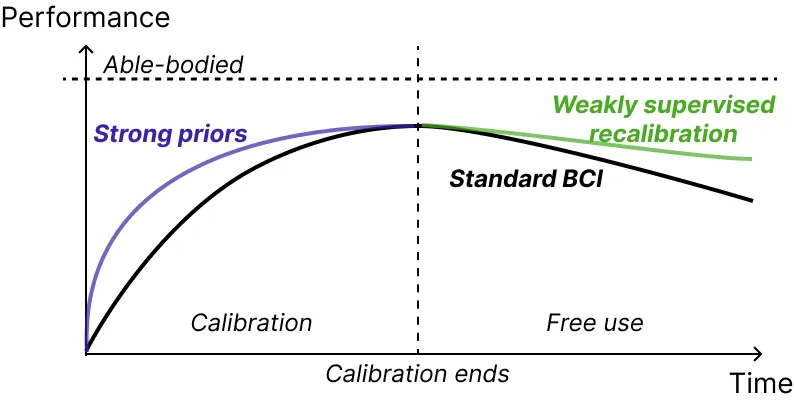
\includegraphics[width=0.5\linewidth]{ch1_ibci_stability.png}
  \caption{iBCI stability challenges.}
  \label{fig:ibci_stability}
\end{figure}

Current somatosensory BCIs are in a pre-paradigmatic state. Plainly, there is no strongly predictive model of what different ICMS patterns will do in a particular individual or implant, so the analogous calibration process is to collect perceptual reports for as many different stimuli as fit within experimental time constraints. The most studied parameterization of ICMS is under fixed-frequency and fixed-amplitude pulse trains on single electrodes. Under this parameterization, the evoked sensation is highly stable over time, but the precise quality and intensity of the sensation can vary across days \citep{citationNeeded}. Worse, the impacts of stimulation frequency and amplitude on these sensations will vary across stimulation electrodes \citep{hughesPlaceholder}. One promising development towards more precise and reliable ICMS is the principle of biomimicry, which motivates the design of stimulation pulses that evoke neural responses resembling those of natural touch. Realizing biomimetic ICMS in higher fidelity through local neural activity will require addressing assumptions on both the neural and perceptual sides.

\section{Deep network models of BCI data}

Modern deep learning typically organizes applications research by the data being modeled, the model architecture, and the optimization objective. The neural data recorded from our BCIs are multichannel voltage time series. In most works here, broadband voltage is filtered and thresholded to extract spikes. A typical BCI dataset includes 100--200 electrode channels with dozens of clearly isolated neurons and many more channels with ``hash'' where non-distinctive spiking waveforms dominate. Behavior in motor datasets is typically recorded as upper limb kinematics or electromyography that varies on the timescale of seconds. Sensory stimuli comprise trains of biphasic current-controlled pulses with variable timing and amplitude.

A great variety of architectures have come and gone, with many performance distinctions waved away by the \emph{Bitter Lesson} \citep{sutton2019}. For this proposal I distinguish two superordinate model classes: recurrent neural networks (RNNs) and Transformers. Transformers feature widely here due to empirical dominance across ML domains, including time series such as audio. Training objectives are primarily prediction-based supervised learning (regression or classification), whether the model is used as a decoder (neural$\rightarrow$behavior), encoder (stimulus$\rightarrow$neural), or representation learner (neural-only).

Two characteristics recur in neural data: (i) large components connected to covariates of interest (e.g., cosine tuning in motor cortex), suggesting simple models can perform well; and (ii) nonstationarity due to cognitive state, electrode--tissue interface, and hardware state, implying the need for robustness to shifts.

A modern phenomenon is that model performance often scales with pretraining on broad data, leading to ``foundation models'' \citep{bommasani2021}. A contingent of neuroscientists seeks to establish a similar paradigm for neural data via large repositories and scaled training. Aim~1 executes precisely this effort for BCI data.

% =========================
% Aim 1
% =========================
\chapter{Aim 1: Large-scale pretraining for intracortical neural datasets}

\section{Summary and Significance}
Deep learning’s greatest successes have depended on exploiting large and varied datasets. We perform two scaling studies on Transformer pretraining for motor cortical decoding, measuring returns on increased pretraining across sessions, subjects, and tasks. Cross-session data scales nearly as well as same-day data, while cross-subject and cross-task data yield positive but attenuated returns. Pretraining on $\sim$2000 hours of pooled activity continues to help, but benefits decline rapidly as downstream data grows (converging near $\sim$90 minutes of task data). Thus, pretraining accelerates calibration but does not eliminate the need for ongoing data collection.

\paragraph{Papers.} Ye et~al., ``Neural Data Transformer 2''; Ye et~al., ``A Generalist Intracortical Motor Decoder.''

\section{Approach}
We study pretraining (large, loosely related datasets) and fine-tuning (small, closely related data) while varying data volume, diversity, model size, and compute. Evaluation uses fixed held-out contiguous blocks per dataset. The NDT2 and NDT3 architectures tokenize spikes in 20\,ms bins and spatial patches; NDT2 follows a masked prediction objective, while NDT3 is autoregressive and supports variable behavioral dimensionality.

\begin{figure}[h]
  \centering
  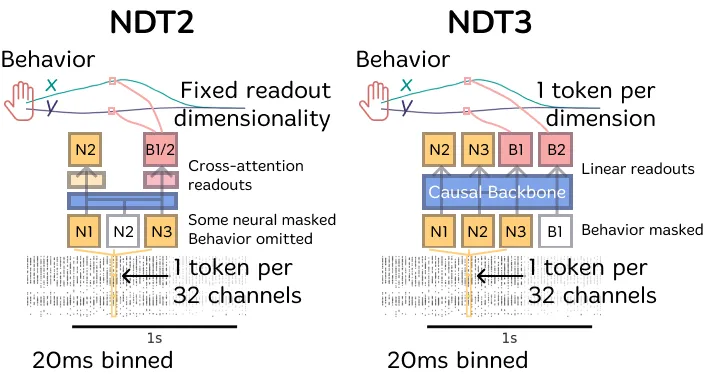
\includegraphics[width=0.5\linewidth]{ch2_ndt_models.png}
  \caption{NDT2 and NDT3 both take input neural data and output neural data and behavior predictions. Both models tokenize neural data in time with 20ms timebins and in space by dividing the population activity into subsets of fixed size (32 in this figure). NDT2 emits one behavior token for prediction at each timestep, while NDT3 emits one behavior token per behavior dimension and timestep, which enables streamlined prediction of behavioral data of varied dimensionality. NDT2, inspired by a Masked Autoencoder design [He], masks out a fraction of neural token inputs and only predicts this fraction. NDT3 adopts the autoregressive modeling framework and allows prediction of all neural tokens conditioned on neural tokens from previous timesteps.}
  \label{fig:ndt_models}
\end{figure}

\section{Results}
NDT2 demonstrates transfer across sessions/subjects/tasks via population patching, Pareto-dominating from-scratch models in zero-shot and with small supervised/unsupervised calibration. NDT3 scales pretraining to 2000\,h and confirms: (i) pretraining helps broadly up to $\sim$90\,min of downstream data, after which from-scratch models catch up; (ii) larger pretraining datasets and models yield better averages.

\begin{figure}[h]
  \centering
  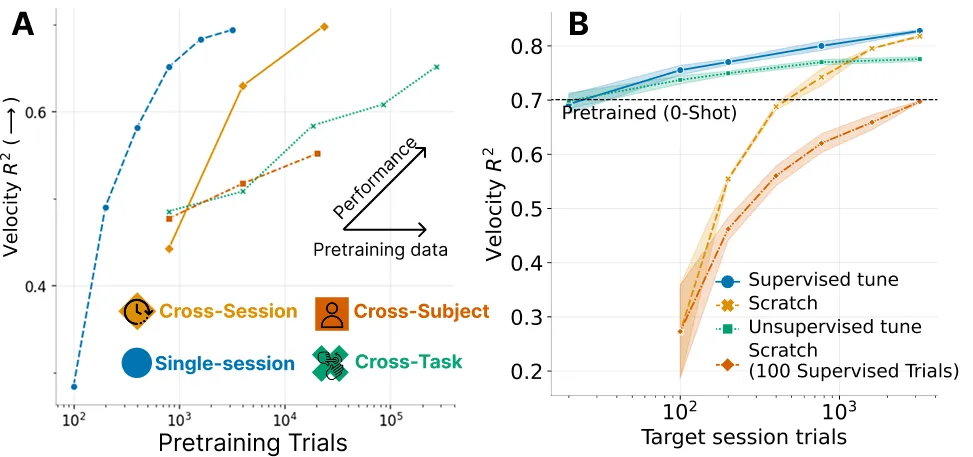
\includegraphics[width=0.5\linewidth]{ch2_ndt2_results.png}
  \caption{A. NDT2 decoding of monkey reach velocity scales with increasing pretraining data from different sessions, subjects, and behavioral tasks. The pretraining abscissa for the single-session curve indicates the total training data available to the model. For the order curves, the abscissa indicates the pretraining data scale. These pretrained models fine-tune to the target session with 100 trials of data. B. Pretrained multisession models can be deployed on new sessions for immediate zero-shot performance. They can also be tuned either through supervised or unsupervised objectives to improve performance, which pareto-dominates performance achieved by training models from scratch.}
  \label{fig:ndt2_results}
\end{figure}

\begin{figure}[h]
  \centering
  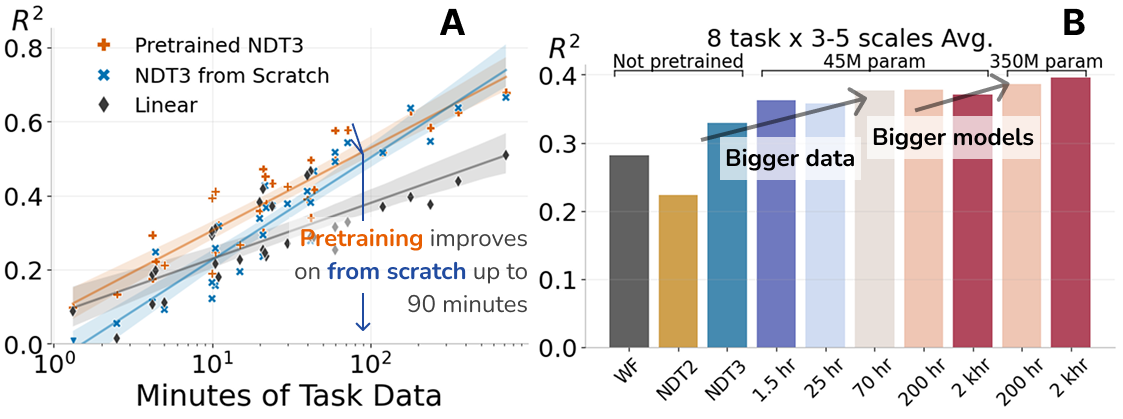
\includegraphics[width=0.5\linewidth]{ch2_ndt3_summary.png}
  \caption{Two summary views of all evaluations conducted on NDT3 models. Left: When evaluations are organized by downstream data scale (Minutes of Task Data), a pretrained model is better than or equal to non-pretrained models and a linear baseline at all data scales. However, the non-pretrained NDT3 model matches the pretrained model when downstream task data is sufficiently large, here at 90 minutes. Right: Collapsing all evaluations into a single average, we see that scaling pretraining dataset size and model size improves summary performance.}
  \label{fig:ndt3_summary}
\end{figure}

\begin{figure}[h]
  \centering
  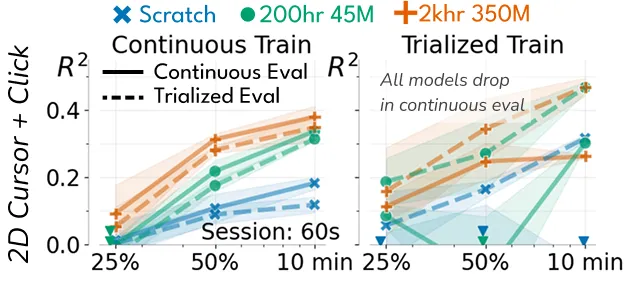
\includegraphics[width=0.5\linewidth]{ch2_trialized.png}
  \caption{Models are evaluated on a human open-loop cursor dataset prepared in two ways. Trialized training receives inputs according to trial boundaries, varying from 2-4 seconds in length. Continuous training receives random 1 second snippets (that can cross trial boundaries). Trialized evaluation matches trialized training, and continuous evaluation is done by streaming up to 1 second of history. Downward arrows indicate points below 0.0. Continuously trained models perform well in both evaluation settings, while models trained on trialized data fail in continuous evaluation.}
  \label{fig:trialized}
\end{figure}

% =========================
% Aim 2
% =========================
\chapter{Aim 2: Pretrained deep networks enable continuous and scalable upper-limb neuroprosthetic control}

\section{Summary and Significance}
Implanted BCIs can decode diverse upper-limb behaviors, but current decoders need substantial daily calibration and underperform able-bodied control. We propose NDT3-based controllers accumulating calibration across days to deliver robust 7--9\,DoF control in up to two participants, and to demonstrate scalability to additional hand DoF without architectural changes.

\section{Approach}
Key ideas: (i) shift from daily retraining to a large initial calibration plus brief daily adaptation; (ii) extend to higher DoF, starting with thumb and grouped fingers. Calibration uses virtual reach--grasp--carry sequences at multiple speeds; training uses robust objectives (e.g., Soft-DTW). Evaluation includes ARAT and timed object transfer, plus virtual metrics (path efficiency, phase-wise performance).

\section{Results \& Remaining Work}
Pilots: NDT3 matches linear decoders for 2D cursor control; ReFIT improves linear speed more than NDT, suggesting gain/label-noise sensitivity. In 4D Mujoco control, linear decoders degrade under unconstrained DoF due to instability, whereas NDT maintains performance via implicit DoF isolation. Multiday adaptation boosts success and completion time, supporting feasibility for continuous 7D control.

\begin{figure}[h]
  \centering
  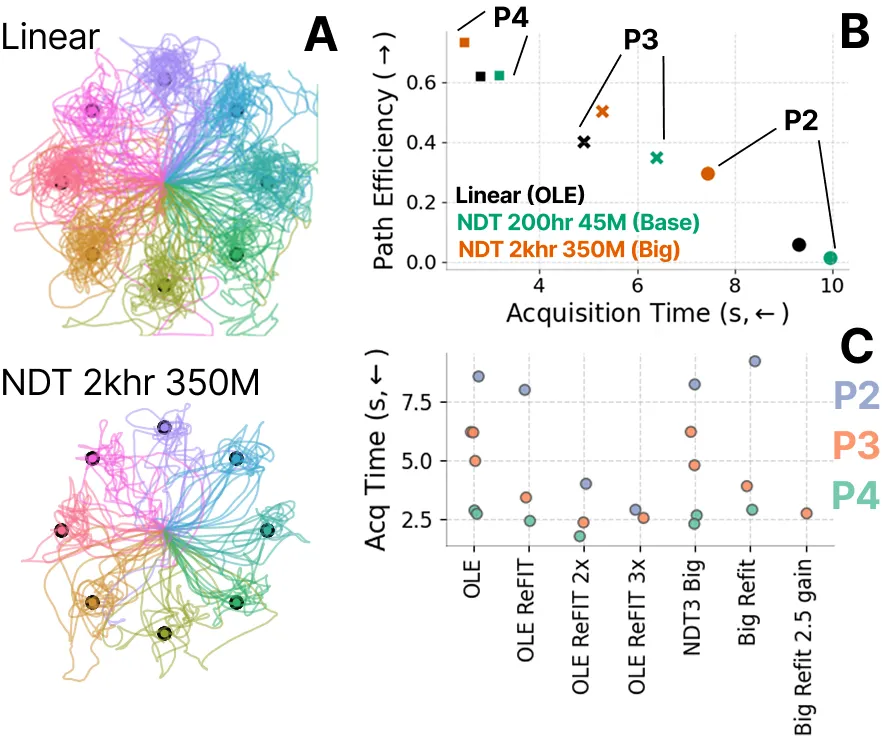
\includegraphics[width=0.5\linewidth]{ch3_cursor_control.png}
  \caption{A. OLE and NDT brain-control trajectories in one human participant. B. NDT matches linear model performance for 2D cursor control when all models are trained on an open loop calibration block. Fitting the large NDT model is preferred. B. After closed loop tuning, linear control steadily improves, but NDT speed does not. Gain can be increased to keep NDT at pace.}
  \label{fig:cursor}
\end{figure}

\begin{figure}[h]
  \centering
  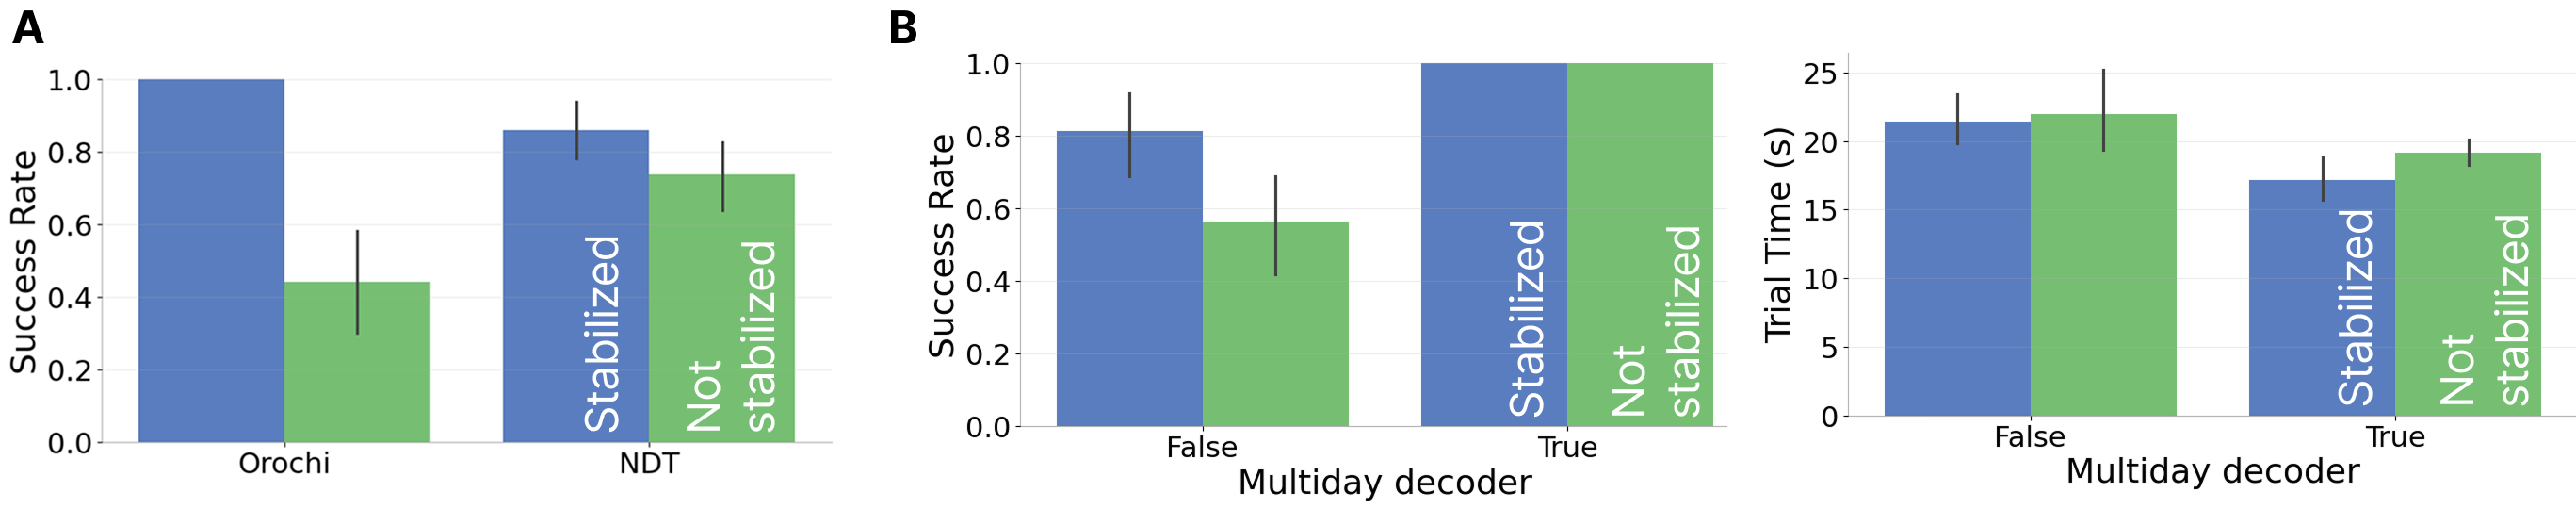
\includegraphics[width=0.5\linewidth]{ch3_mujoco_results.png}
  \caption{A. Orochi linear decoder compared against NDT DNN decoder for Mujoco 4D FBC Sequenced movement trials. Error bars show standard deviation across trials. Evaluations are conducted in constrained and unconstarined settings. Constrained evaluations only allow one of arm translation, wrist rotation, or hand grasp to be active at a time. B. Multiday NDT decoders achieve high success and faster completion times relative to decoders trained from scratch.}
  \label{fig:mujoco}
\end{figure}

% =========================
% Aim 3
% =========================
\chapter{Aim 3: Modeling the neural response to intracortical microstimulation}

\begin{figure}[h]
  \centering
  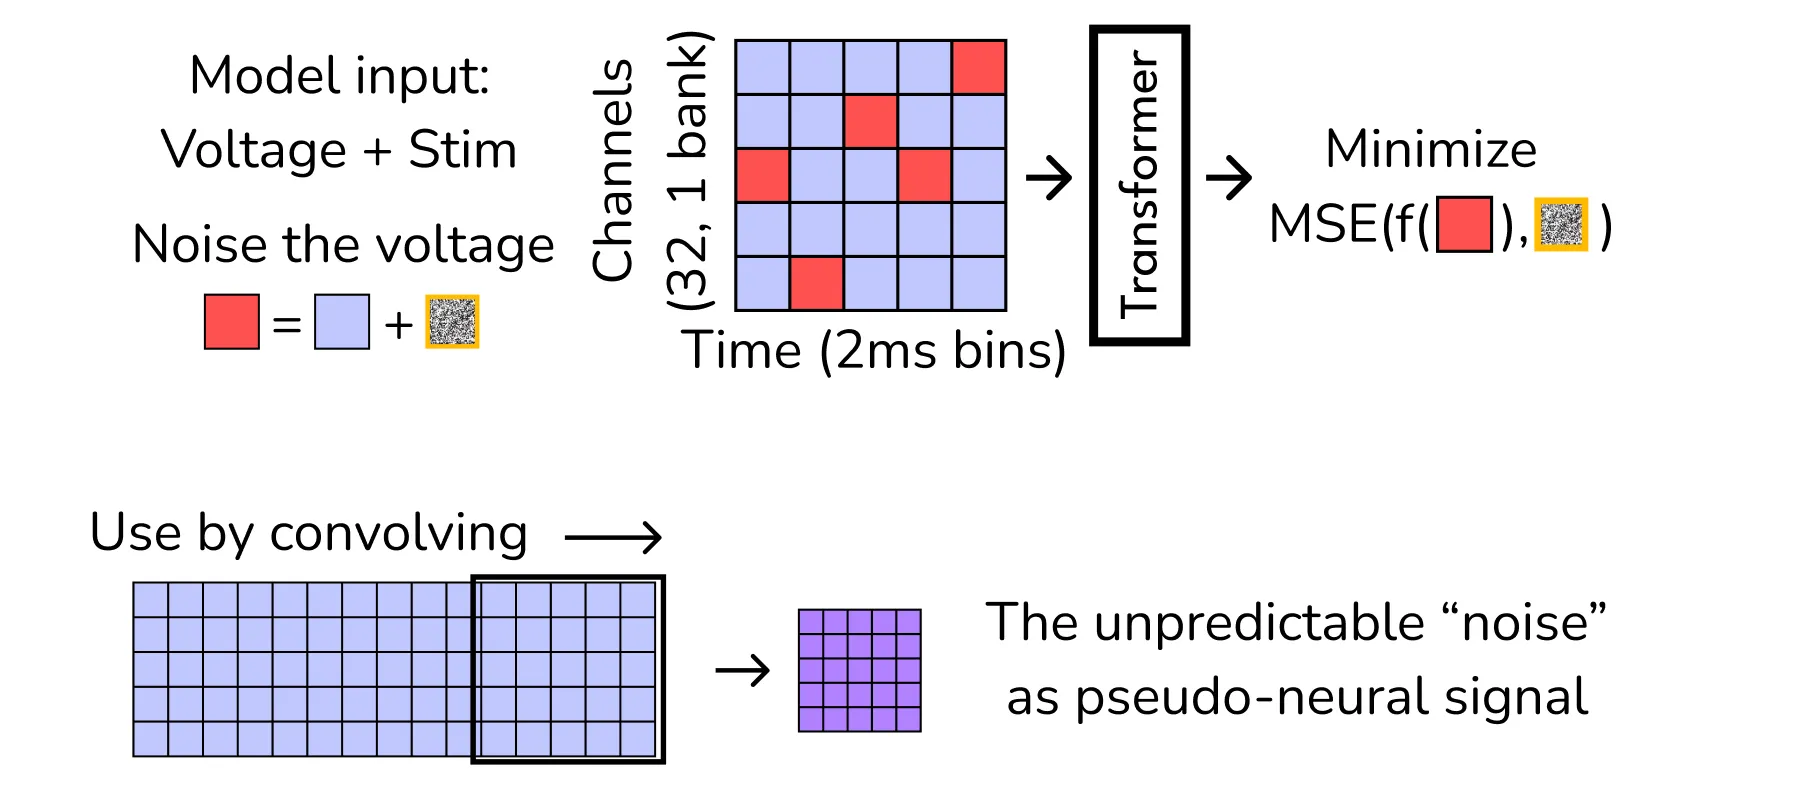
\includegraphics[width=0.5\linewidth]{ch4_delete_schema.png}
  \caption{DELETE method schematic overview.}
  \label{fig:delete_schema}
\end{figure}

\begin{figure}[h]
  \centering
  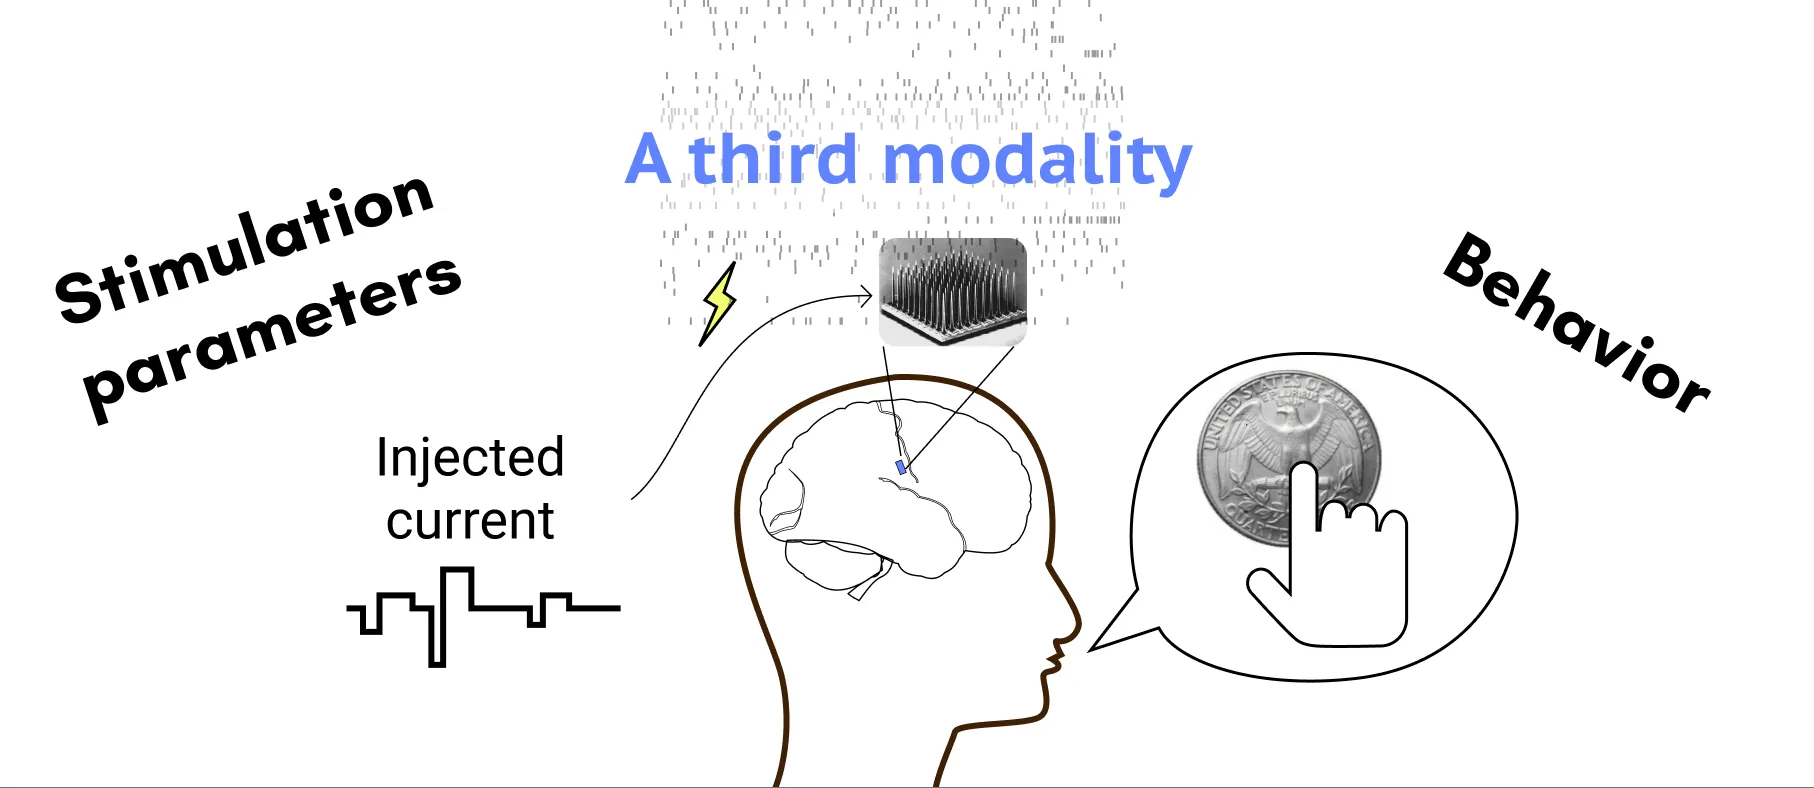
\includegraphics[width=0.5\linewidth]{ch4_third_modality.png}
  \caption{Third modality analysis for ICMS modeling.}
  \label{fig:third_modality}
\end{figure}

\section{Summary and Significance}
Sensory feedback is integral to dexterous control. We decompose the stimulation problem into modeling (i) stimulation$\to$local neural response and (ii) local response$\to$percept. We focus here on (i), introducing DELETE (Denoising Electrical Events with a Transformer Encoder) for artifact removal and using transfer-learning assays to taxonomize ICMS responses across temporal patterns and channels.

\section{Approach}
\subsection*{Recovering the neural response with DELETE}
DELETE reconstructs broadband multichannel activity to estimate and subtract artifacts. Constraints (short windows, point-estimate loss, broad training) reduce the risk of erasing spikes. We benchmark DELETE against PCA/linear baselines and analyze as a generic denoiser on non-ICMS data.

\begin{figure}[h]
  \centering
  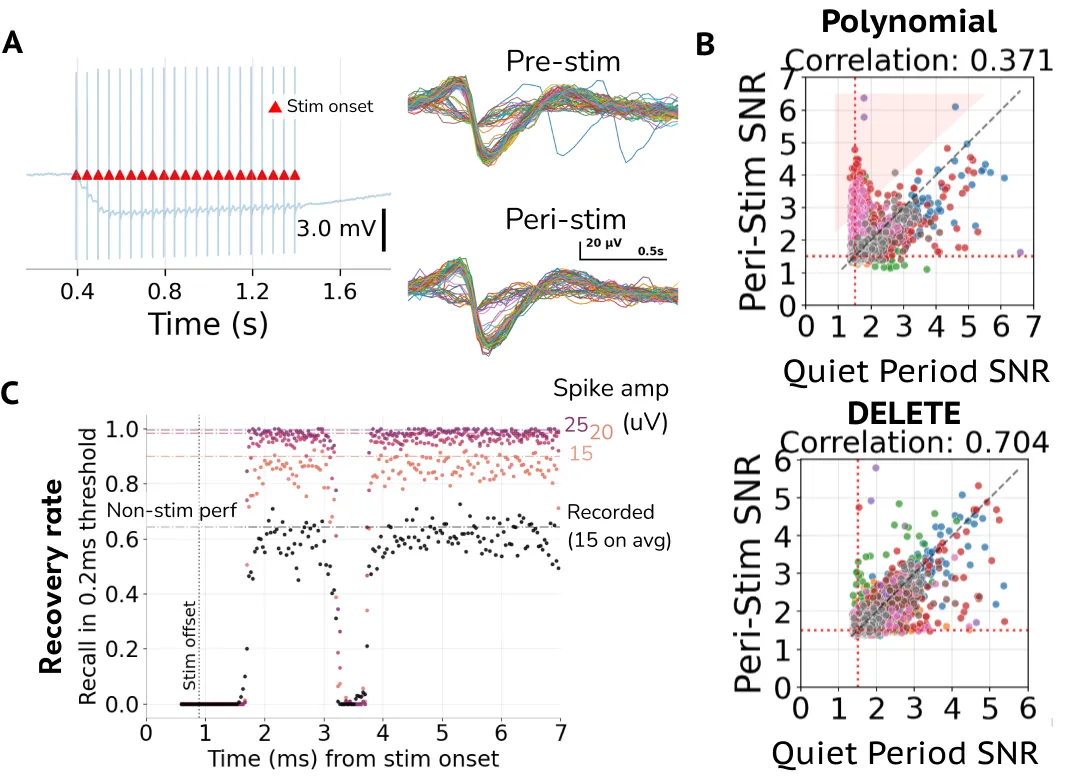
\includegraphics[width=0.5\linewidth]{ch4_delete_peristim.png}
  \caption{A. Left: A sample broadband recording from a channel during a stimulation trial. The displayed channel is on the electrode array that is stimulated. Right: Spike waveforms recovered from the broadband activity both prior to stimulation onset and in the artifacted peri-stimulation period. B. To summarize waveform recovery, we compute channel SNR as a ratio of peak waveform amplitude against background noise amplitude. The color of each dot indicates the physical array the channel is on. We expect physiological waveform SNRs to be conserved through stimulation, so high correlation of quiet period and peri-stim SNR provides a heuristic for good de-artifacting. Dashed red lines indicate the 4.5x background noise threshold we use to determine spike presence. C. We evaluate model sensitivity by injecting synthetic spikes into the broadband activity and evaluating whether they are recovered. The colored curves differ in the precise waveform injected, which were either recorded and extracted from the data or simulated. Horizontal lines indicate the noise ceiling computed as the recovery rate of spikes injected outside of stimulation periods.}
  \label{fig:delete_peristim}
\end{figure}

\subsection*{Taxonomizing passive ICMS responses}
We collect single- and multi-channel passive ICMS datasets including random-amplitude Poisson (RAP) and fixed-train stimuli, and use RNN/Transformer models to test generalization across time patterns, channels, and days.

\begin{figure}[h]
  \centering
  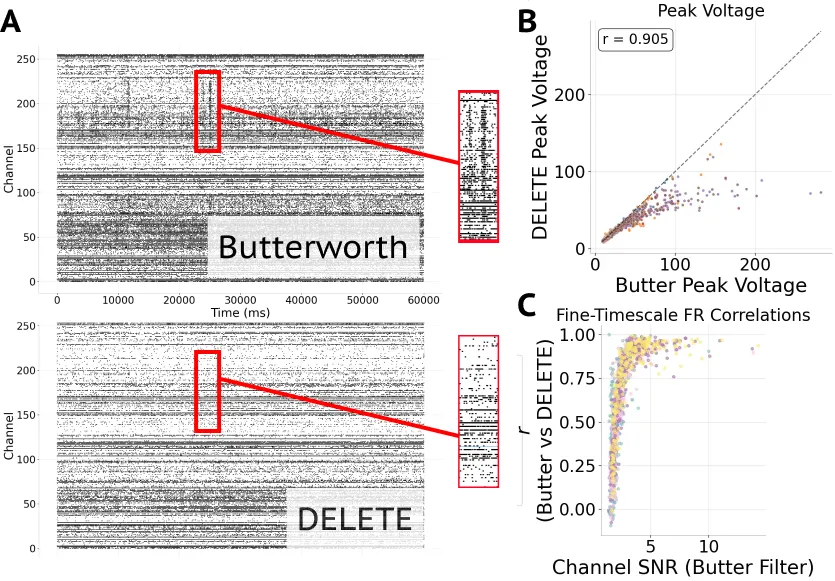
\includegraphics[width=0.5\linewidth]{ch4_delete_generic.png}
  \caption{A. Top: Butteworth filter extracted spiking activity from a minute of resting state recordings. Inset shows putative movement-induced artifact. Bottom: The same data pre-filtered by DELETE, inset no longer shows correlated firing across channels. B. Peak voltages of waveforms extracted by DELETE and a standard Butterworth filter are compared. There is high correlation, but DELETE peaks saturate by 100uV. C. Firing rates are determined by convolving a 50ms Gaussian kernel against Butterworth or DELETE filtered spiking activity. These per-channel firing rates are correlated across a number of different channels and datasets. Color of dots indicate datasets. High SNR channels correlate well.}
  \label{fig:delete_generic}
\end{figure}

\begin{figure}[h]
  \centering
  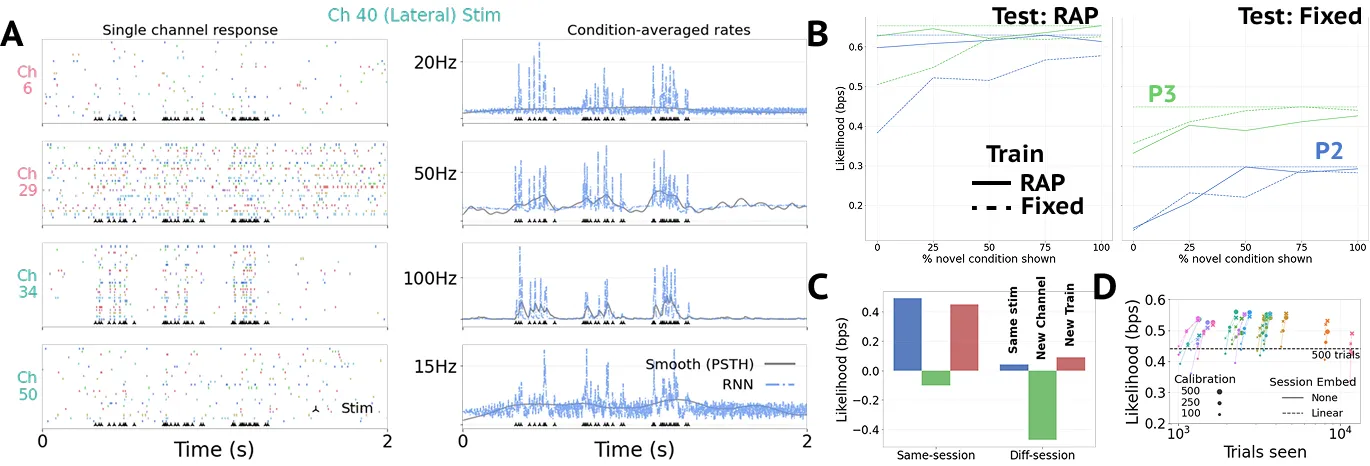
\includegraphics[width=0.5\linewidth]{ch4_icms_taxonomy.png}
  \caption{A. Example raster plots to stimulation on a single channel (40). Modulated responses are visible both on the stimulated array (bottom two rows) and another sensory array (top two rows). Firing rates as inferred by computing PSTH and RNN models are given on the right. B. Example analysis testing generalization of RNN models to novel single channel stimulation trains. In these plots, models are first trained on either random amplitude Possion (RAP) or fixed frequency and amplitude trains (Fixed). They are then gradually exposed to increasing levels (\% novel condition shown) of a new set of ICMS again from either RAP or fixed stimuli (Test condition). The flat dotted line marks the max performance achieved by any in-distribution model. The closer the other curves are to this flat line, the better the model's generalization to new stimuli. C. Here, we train one model on one type of RAP ICMS and assess its generalization to 3 stimulation conditions from either the same or different experimental session. D. We conduct a brief scaled pretraining analysis. We vary the pretraining scale (Trials seen) and subsequent fine-tuning scale (Calibration), and evaluate on a new session. Session identity is either not modeled (Session Embed None) or modeled with a linear readin layer (Linear). The reference line shows session performance using only 500 calibration trials from the evaluation dataset. Most pretrained models exceed this level, suggesting positive transfer.}
  \label{fig:icms_taxonomy}
\end{figure}

\section{Results \& Remaining Work}
DELETE outperforms baselines for peri-stim recovery and preserves high-SNR spike statistics on non-ICMS data. ICMS taxonomy suggests temporal-pattern generalization within-channel is good (RAP$\to$RAP), but cross-channel transfer is weak; multiday models benefit from increased training data but can plateau or regress with RNNs, motivating NDT-style multisession models. Remaining work: finalize DELETE benchmarking suite; ground recovered response statistics physiologically; expand taxonomy across participants/areas or toward inverse-modeling/percept decoding.

% =========================
% Schedule
% =========================
\chapter{Schedule}
Aim~3 started first but paused for dataset aggregation work. Next steps: collect NDT-control data and write results; then finish DELETE and ICMS taxonomy as two publications.

\begin{figure}[h]
  \centering
  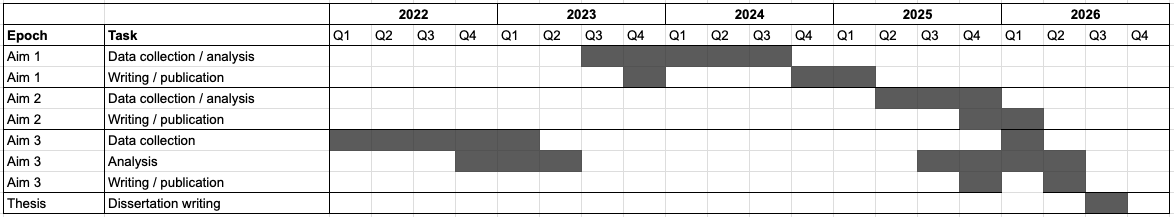
\includegraphics[width=0.5\linewidth]{ch5_schedule_gantt.png}
  \caption{High-level schedule/Gantt (placeholder: \texttt{figures/schedule\_gantt.png}).}
  \label{fig:schedule}
\end{figure}

% =========================
% References
% =========================
\cleardoublepage
\printbibliography

\end{document}
